\section{Introduction}
%what is the problem
Data indexing is an important component of any practical data storage system/DBMS.
A data index essentially accelerates the read path of the data store by maintaining
fast metadata lookup for already written/stored data. However, the index itself 
needs to be persistent in addition to the stored data. Persistent index enables 
instant recovery for the DBMS as we do not have to rebuild the index from scratch.

Maintaining consistent persistent index has its own overheads. First, we have to keep 
index updated, to keep correctness between index and the data it points to. We identify
this as runtime-consistency. Next, we should make sure that, our index remain consistent
even after a unplanned system crash.That is, during index updates we have to maintain
all-or-nothing semantics by using some form of logging protocol (e.g. Aries).


Furthermore maintaining persistent index for block based storage is challenging.
First, disk I/O based DBMS system (e.g. SSD) access data in blocks. That is 
even if you are accesing one byte of data, you have to bring in the whole block in to the
volatile memory. Second, these devices have low access latency compared to volatile main memory --
two orders of magnitude slower than DRAM. Therefore, the disk based persistent indexes are
stored out of band (in a seperate file structure) from the actual data. This design
decision benefits the index traveral. This is because, such data organization enables
maximum index data availability on volatile buffer-caches.


\section{Motivation}
%why is this problem important
Non volatile memory(NVM) is an emerging storage technology that promises byte addressable 
persistency. NVMs have read/write latencies that are comparable to DRAM and the device 
writes are durable. Fast accesses latencies and byte addressablity enables this new device
to be placed alongside with DRAM main memory, thus providing direct persistent load/stores
from the processor. Furthermore NVMs have high form factor (high capacity devices) thus
making them ideal devices for both persistent index and data storage. However, naive port
of existing persistent indexes structures on to NVM is not going to yield the best performance.

First, some of the assumptions that were made during the design of disk oriented persistent
indexes does not hold true anymore, 1) We can access NVM resident data at byte granularity similar to
DRAM data acesses. 2) The NVMs provide load store accesses at DRAM speed. Therefore, we can
possibly store index, alongside the actual data as the index retrival is not slowed down by
accompanying data. Furthermore, the use of DRAM buffer-cache is redundant as the NVMs are 
as good as DRAM in terms of access latency.

Next, persistent programming on NVMs is non-trivial task. Specifically, unlike volatile memory
data strucrures, the NVM writes are durable across system restarts. Therefore, care should be
taken when updating NVM resident persistent index to maintain both runtime and crash consistency.
The existing main memory indexes already provide addresses efficient runtime consistent state 
maintenance. However, they lack the crash-consistency semantics. While NVM itself is persistent,
when accessed via CPU's load/store interface the writes get cached in the processor's volatile
caches -- that re-orders the writes on to NVM. We have to explicitly order the writes on to NVM
to do crash-consistent updates.


Finally, while NVMs provide fast read/write accesses, the they have assymetric performance 
characteristics -- NVM reads are cheaper than NVM writes. NVM writes involve changing physical
state of the device and thus exepensive interms of energy and latency. NVM aware persistent 
index design should take the read/write assymetry in to account for an NVM friendly data
structure design.

\section{NVStore}
%proposed solution

We propose NVStore, a persistent key-value store that is based on NVM aware persistent index
structure. 

\subsection{Zero-copy Index}

First, we store NVStore key-value pairs in a log-structured memory segments on NVM. These, are 
formatted in to C like memory structures, that gets sequentially stored on the log-segments. The
C-structure based key-value storage allows direct referencing/de-referencing of stored data 
as regular memory structures. The log-structuring of groups of such structures allow us to 
exploit the superior sequential performance of the NVM device.

Next, offload some of the metadata maintainance in to data nodes itself. This is a viable
option becauseo of low latency random accesses supported by




\begin{figure}[]   
	\centering
	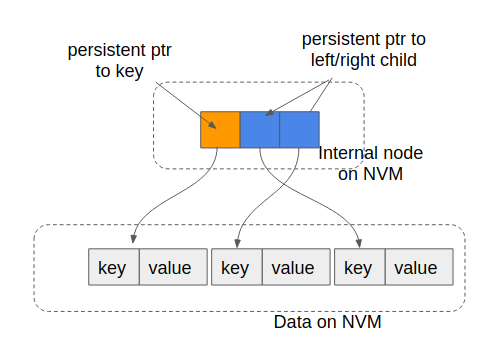
\includegraphics[width=\linewidth]{figures/zerocopy.png} 
	\caption{\bf Node structure of a RBTree node. We do not store key vlaues in the internal nodes. We simply
	store a persistent pointer in to the external key.} 
	\label{fig:zerocopy} 
\end{figure}

\subsection{Crash-consistent Index Updates}

\cite{pmwcas}
